\documentclass{article}[18pt]
\ProvidesPackage{format}
%Page setup
\usepackage[utf8]{inputenc}
\usepackage[margin=0.7in]{geometry}
\usepackage{parselines} 
\usepackage[english]{babel}
\usepackage{fancyhdr}
\usepackage{titlesec}
\hyphenpenalty=10000

\pagestyle{fancy}
\fancyhf{}
\rhead{Sam Robbins}
\rfoot{Page \thepage}

%Characters
\usepackage{amsmath}
\usepackage{amssymb}
\usepackage{gensymb}
\newcommand{\R}{\mathbb{R}}

%Diagrams
\usepackage{pgfplots}
\usepackage{graphicx}
\usepackage{tabularx}
\usepackage{relsize}
\pgfplotsset{width=10cm,compat=1.9}
\usepackage{float}

%Length Setting
\titlespacing\section{0pt}{14pt plus 4pt minus 2pt}{0pt plus 2pt minus 2pt}
\newlength\tindent
\setlength{\tindent}{\parindent}
\setlength{\parindent}{0pt}
\renewcommand{\indent}{\hspace*{\tindent}}

%Programming Font
\usepackage{courier}
\usepackage{listings}
\usepackage{pxfonts}

%Lists
\usepackage{enumerate}
\usepackage{enumitem}

% Networks Macro
\usepackage{tikz}


% Commands for files converted using pandoc
\providecommand{\tightlist}{%
	\setlength{\itemsep}{0pt}\setlength{\parskip}{0pt}}
\usepackage{hyperref}

% Get nice commands for floor and ceil
\usepackage{mathtools}
\DeclarePairedDelimiter{\ceil}{\lceil}{\rceil}
\DeclarePairedDelimiter{\floor}{\lfloor}{\rfloor}

% Allow itemize to go up to 20 levels deep (just change the number if you need more you madman)
\usepackage{enumitem}
\setlistdepth{20}
\renewlist{itemize}{itemize}{20}

% initially, use dots for all levels
\setlist[itemize]{label=$\cdot$}

% customize the first 3 levels
\setlist[itemize,1]{label=\textbullet}
\setlist[itemize,2]{label=--}
\setlist[itemize,3]{label=*}

% Definition and Important Stuff
% Important stuff
\usepackage[framemethod=TikZ]{mdframed}

\newcounter{theo}[section]\setcounter{theo}{0}
\renewcommand{\thetheo}{\arabic{section}.\arabic{theo}}
\newenvironment{important}[1][]{%
	\refstepcounter{theo}%
	\ifstrempty{#1}%
	{\mdfsetup{%
			frametitle={%
				\tikz[baseline=(current bounding box.east),outer sep=0pt]
				\node[anchor=east,rectangle,fill=red!50]
				{\strut Important};}}
	}%
	{\mdfsetup{%
			frametitle={%
				\tikz[baseline=(current bounding box.east),outer sep=0pt]
				\node[anchor=east,rectangle,fill=red!50]
				{\strut Important:~#1};}}%
	}%
	\mdfsetup{innertopmargin=10pt,linecolor=red!50,%
		linewidth=2pt,topline=true,%
		frametitleaboveskip=\dimexpr-\ht\strutbox\relax
	}
	\begin{mdframed}[]\relax%
		\centering
		}{\end{mdframed}}



\newcounter{lem}[section]\setcounter{lem}{0}
\renewcommand{\thelem}{\arabic{section}.\arabic{lem}}
\newenvironment{defin}[1][]{%
	\refstepcounter{lem}%
	\ifstrempty{#1}%
	{\mdfsetup{%
			frametitle={%
				\tikz[baseline=(current bounding box.east),outer sep=0pt]
				\node[anchor=east,rectangle,fill=blue!20]
				{\strut Definition};}}
	}%
	{\mdfsetup{%
			frametitle={%
				\tikz[baseline=(current bounding box.east),outer sep=0pt]
				\node[anchor=east,rectangle,fill=blue!20]
				{\strut Definition:~#1};}}%
	}%
	\mdfsetup{innertopmargin=10pt,linecolor=blue!20,%
		linewidth=2pt,topline=true,%
		frametitleaboveskip=\dimexpr-\ht\strutbox\relax
	}
	\begin{mdframed}[]\relax%
		\centering
		}{\end{mdframed}}
\lhead{CSys - Databases}


\begin{document}
\begin{center}
\underline{\huge The Entity Relationship Model}
\end{center}
\section{Why a data model?}
\begin{itemize}
\item A model: an abstract representation of something existing in the real world
\item Models help make complex things understandable
\item In databases:
\begin{itemize}
\item DDL is too low level
\item not easily understandable by most users
\end{itemize}
\item We have seen:
\begin{itemize}
\item Relational data model
\item Relations between data $\rightarrow$ stored in tables
\item based on the concept of mathematical relations
\end{itemize}
\end{itemize}
\section{Entity-Relationship Model}
\begin{itemize}
\item Relational data model
\begin{itemize}
	\item Sometimes still too low level for big companies
	\item we need a model of communication that is non technical and free of ambiguities
\end{itemize}
\item Entity relationship model - a graphical description of the DB
\item A \textbf{top down} approach to database design
\begin{itemize}
	\item Start with a set of requirements
	\item identify the types of "things" that you need to represent data about
	\item Identify the attributes of those "things"
\end{itemize}
\item Objective of the ER model
\begin{itemize}
	\item To help understanding of the nature and relationships among the data
	\item To help deriving the tables in the relational data model
\end{itemize}
\item Most important before building the ER model:
\begin{itemize}
	\item proper understanding of the problem domain (the scenario)
	\item lack of understanding $\rightarrow$ wrong ER model $\rightarrow$ wrong DB design
\end{itemize}
\item Basic concepts:
\begin{itemize}
	\item the important data objects (entities)
	\item the important properties of the entities (attributes)
	\item the associations between the entities (relationships)
\end{itemize}
\item Furthermore - constraints on the entities, relationships and attributes
\item Several notations for representing the ER model:
\begin{itemize}
	\item Crow's foot notation
	\item UML notation (unified modelling language)
\end{itemize}
\end{itemize}
\section{Main components of an ER model}
\begin{itemize}
	\item An entity
	\begin{itemize}
		\item any real thing that we recognise as a separate concern within the database
		\item important enough to be represented separately
		\item A rectangle represents an entity type
	\end{itemize}
	\item Relationship
	\begin{itemize}
		\item A named association between two entity types
		\item Shown by a labelled line connecting two entities 
	\end{itemize}
\end{itemize}
\section{Cardinality}
\begin{itemize}
	\item The cardinality of a relationship - the number of entity occurrences that are related to a single occurence of an associated entity type through this relationship
	\item The cardinality of a relationship can be
	\begin{itemize}
		\item one to one
		\item one to many
		\item many to many
	\end{itemize}
\end{itemize}
Many to one is not needed, as it is just the opposite way round as one to many.
\section{Optionality and participation}
\begin{itemize}
	\item Optionality is where a relationship could or could not exist, and is denoted by a circle in the ER diagram
\begin{center}
	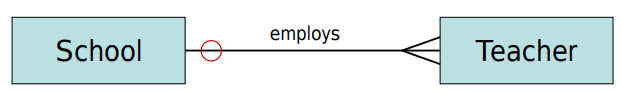
\includegraphics[scale=0.7]{optionality}
\end{center}
	\item if an entity participates optionally in a relationship:
	\begin{itemize}
		\item it has partial participation
		\item otherwise it has total participation
	\end{itemize}
	\item In the ER diagram total participation is denoted by a vertical bar
	\begin{center}
		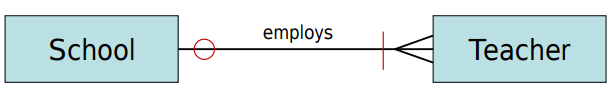
\includegraphics[scale=0.7]{participation}
	\end{center}
	
\end{itemize}
\section{Attributes}
\begin{itemize}
	\item The attributes of an entity
	\begin{itemize}
		\item The set of all common characteristics that are shared by all entity occurrences of an entity type
	\end{itemize}
	\item Diagrammatic representation of attributes have primary keys underlined
	\begin{itemize}
		\item for every attribute one \textbf{labeled ellipse} attached to the entity rectangle
		\item all attributes in the lower part of the entity rectangle
	\end{itemize}
\end{itemize}
\subsection{Determining the attributes}
What are the appropriate attributes
\begin{itemize}
	\item We first look for the natural characteristics of an entity
	\item an attribute can be associated with a value domain
	\item Single value attribute - holds only one value
	\item Multivalued attribute - holds many values
	\item Derived attribute - derivable from the value of a related attribute
\end{itemize}
\section{Step by step construction of an ER model}
\begin{enumerate}
	\item Identify entities from the scenario/real world
	\item Find relationships
	\item Draw rough ER diagram
	\item Fill in the relationships
	\item Define primary keys and resolve many to many relationships
	\item Identify attributes and map them to the entities
	\item Draw full ER diagram showing keys, attributes, relationships
	\item Check it reflects the real world system
\end{enumerate}
\end{document}